% Template for Cogsci submission with R Markdown

% Stuff changed from original Markdown PLOS Template
\documentclass[10pt, letterpaper]{article}

\usepackage{cogsci}
\usepackage{pslatex}
\usepackage{float}
\usepackage{caption}

% amsmath package, useful for mathematical formulas
\usepackage{amsmath}

% amssymb package, useful for mathematical symbols
\usepackage{amssymb}

% hyperref package, useful for hyperlinks
\usepackage{hyperref}

% graphicx package, useful for including eps and pdf graphics
% include graphics with the command \includegraphics
\usepackage{graphicx}

% Sweave(-like)
\usepackage{fancyvrb}
\DefineVerbatimEnvironment{Sinput}{Verbatim}{fontshape=sl}
\DefineVerbatimEnvironment{Soutput}{Verbatim}{}
\DefineVerbatimEnvironment{Scode}{Verbatim}{fontshape=sl}
\newenvironment{Schunk}{}{}
\DefineVerbatimEnvironment{Code}{Verbatim}{}
\DefineVerbatimEnvironment{CodeInput}{Verbatim}{fontshape=sl}
\DefineVerbatimEnvironment{CodeOutput}{Verbatim}{}
\newenvironment{CodeChunk}{}{}

% cite package, to clean up citations in the main text. Do not remove.
\usepackage{cite}

\usepackage{color}

% Use doublespacing - comment out for single spacing
%\usepackage{setspace}
%\doublespacing


% % Text layout
% \topmargin 0.0cm
% \oddsidemargin 0.5cm
% \evensidemargin 0.5cm
% \textwidth 16cm
% \textheight 21cm

\title{Preserved Structure Across Vector Space Representations}

\usepackage{lipsum}

\author{{\large \bf Andrei Amatuni} \\ \texttt{andrei.amatuni@duke.edu} \\ Department of Psychology \\ Duke University \And {\large \bf Elika Bergelson} \\ \texttt{elika.bergelson@duke.edu} \\ Department of Psychology \\ Duke University}

\begin{document}

\maketitle

\begin{abstract}
We find evidence of preserved structure between vector space
representations of words and their corresponding image embeddings. This
is evidence of regularity between the representations learned using
distributional statistics of words and the visual characteristics of
those same items. We find that some classes of objects, namely inanimate
ones, preserve their within-class structure across these two spaces more
strongly than others (e.g.~animate objects), and that this quality of
preserving class-level relationships across representational spaces
might aid in lexical acquisition, with invariance serving as an
informative marker of category boundaries. Our current analysis does not
show significant AoA benefits for inanimate objects, but does exhibit a
stable pattern suggesting that other partitioning schemes might be worth
exploring (or something like that)

\textbf{Keywords:}
vector space models; semantic similarity; word learning
\end{abstract}

\section{Introduction}\label{introduction}

\section{Methods}\label{methods}

We generate two sets of vector representations for a common set of words
first learned by most infants. The first set of vectors are taken from a
pretrained set of GloVe representations (Pennington, Socher, \& Manning,
2014), a modern distributional semantic vector space model. The second
set is taken from the final layer activations of a pretrained image
recognition model, Google's Inception V3 convolutional neural network
(Szegedy, Vanhoucke, Ioffe, Shlens, \& Wojna, 2016). Both of these
representations are what's refered to as ``embeddings''. They map
objects from one medium (e.g.~images or words) into a metric space,
where distances between points can be computed and function as a measure
of similarity between objects.

In the case of our word vectors, the GloVe algorithm instantiates the
distributional hypothesis, which proposes that words which co-occur with
each other share similar meaning (Firth, 1957; Harris, 1954), and by
capturing the covariance of tokens in large text corpora, you capture
some aspect of their semantic structure. The image embeddings, on the
other hand, are taken from the final layer of activations in a
convolutional neural network, whose objective function tunes network
parameters in service of object recognition, where the loss function is
computed in reference to a set of labeled training images (Russakovsky
et al., 2015). The final layer of this network encodes the most abstract
and integrated visual features, serving as the basis for classification
into 1000 different classes.

\subsection{Defining a prototypical
image}\label{defining-a-prototypical-image}

In the case of word vectors, each word is assigned a unique point in a
common vector space. Different images containing objects of the same
type, on the other hand, will have varying vector representations after
passing through the layers of a neural network. This presents a problem
in comparing the two forms of representation. We must first define the
most prototypical (or average) image vector for any given category of
object.

Given a set of images \(S_c\) containing objects belonging to a single
category \(c\) (e.g.~cat, dog, chair), we define our prototypical vector
\(\hat{x}_c\) of \(S_c\) as the generalized median within a
representational space \(U\). This is the vector with minimal sum of
distances between it and all the other members of set \(S_c\) in \(U\).
If \(x\) and \(y\) are vectors in space \(U\), resulting from images in
\(S_c\) being passed through a neural network, then

\[
 \hat{x_c} = \operatorname*{arg\,min}_{x\in U} \sum_{y\in U} d(x, y)
\] We define our \(d(x, y)\) to be the cosine similarity measure:

\[
d(x, y) = 1 - \frac{x\cdot y}{\|x\|\|y\|}
\]

Our \(d(x, y)\) is not a metric in the strict sense, but is less
susceptible to differences in \(L^2\) norm influencing our measure of
similarity, as is the case with the Euclidean distance. These magnitude
difference can be the product of frequency effects in the training data,
and the cosine similarity corrects for this.

The image inputs we use are all 960x960 images of a single object on a
gray background. These images were chosen by virtue of their presence in
infants' early linguistic environment, aggregated as part of the
SEEDLingS project, which gathered longitudinal audio and video data of
infants' home environments (Bergelson, 2016a, 2016b). We arrive at a set
of 27 unique words, selected on the basis of having at least 9 unique
images with which to determine the most prototypical. The more images we
have of any given category, the more robust our measure of category
variance in image vector space, resulting more representative category
vectors. These are all words found on WordBank (Frank, Braginsky,
Yurovsky, \& Marchman, 2017), a compilation of the MacArthur-Bates
Communicative Development Inventory, which we use as our proxy for age
of acquisition. By studying the behavior of these developmentally
salient objects, our analysis is able to speak to the statistical
structure of those objects which infants will be most readily contending
with.

\subsection{Comparing spaces}\label{comparing-spaces}

After we have our two sets of vectors (i.e.~those from word vector space
and those from image vector space), we can compare all the pairwise
distances between objects, both within a single space and across the
two. When comparing across the two spaces, a correlation in pairwise
distances implies that inter-object distances have been conserved. For
example, if ``dog'' and ``cat'' are close together in word space and
mutually far apart from ``chair'' and ``table'' in that same space,
maintaining this relationship for all pairwise distances in the
\textit{other} vector space means that the global inter-object structure
is preserved across this mapping, despite being in radically different
spaces, both in terms of dimensionality (300 for words, and 2048 for
images in our case) and by virtue of using completely different
algorithms and inputs to establish the vector representations for
objects. So while their absolute locations might have been radically
transformed, this correlation would be a measure of the
\textit{degree of invariance} in their positioning relative to each
other.

\section{Results}\label{results}

We find that pairwise cosine distances between objects in word vector
space correlate with those same pairwise distances in the image vector
space. If we partition the set of inter-word distances into those that
are either animate-animate, inanimate-inanimate, or mixed, we find that
the pairs of distances between inanimate objects significantly correlate
across our two spaces (\(R = 0.38\), \(p < 1.7e-07\)), while the other
two pairings do not.

\begin{CodeChunk}
\begin{figure}[tb]
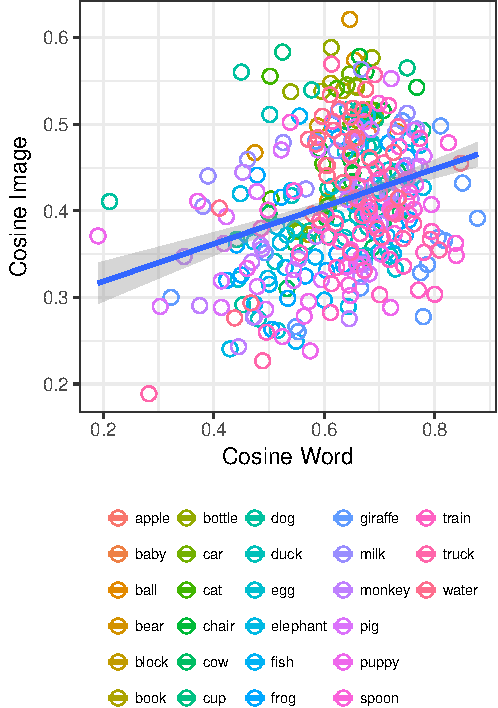
\includegraphics{figs/pairwise_corr-1} \caption[Relative cosine distance between points in word embedding space correlates with relative distance in image embedding space ($R = 0.30$, $p < 9.9e-16$)]{Relative cosine distance between points in word embedding space correlates with relative distance in image embedding space ($R = 0.30$, $p < 9.9e-16$). Graph contains all pairwise distances for every word.}\label{fig:pairwise_corr}
\end{figure}
\end{CodeChunk}

\begin{CodeChunk}
\begin{figure}[tb]
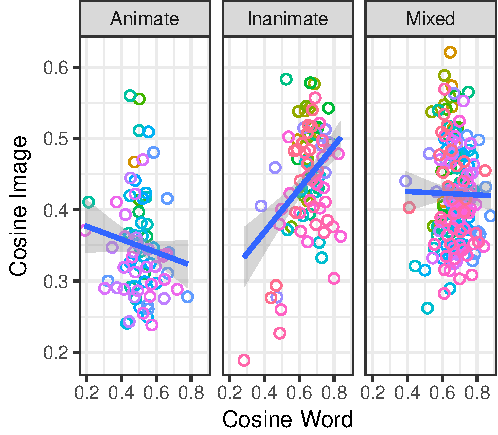
\includegraphics{figs/pairwise_corr_animate_vs_not-1} \caption[Inanimate objects display a significantly stronger correlation when mapping across vector spaces, meaning that they preserve their within-class structural relationships more reliabily across these two spaces]{Inanimate objects display a significantly stronger correlation when mapping across vector spaces, meaning that they preserve their within-class structural relationships more reliabily across these two spaces. Animate and mixed distances do not correlate. Each graph contains all pairwise distances between objects that are either a) both animate ($R = -0.13$, $p < 0.12$), b) both inanimate ($R = 0.38$, $p < 1.7e-07$), or c) mixed animate-to-inanimate ($R = -0.01$, $p < 0.8$)}\label{fig:pairwise_corr_animate_vs_not}
\end{figure}
\end{CodeChunk}

\begin{CodeChunk}

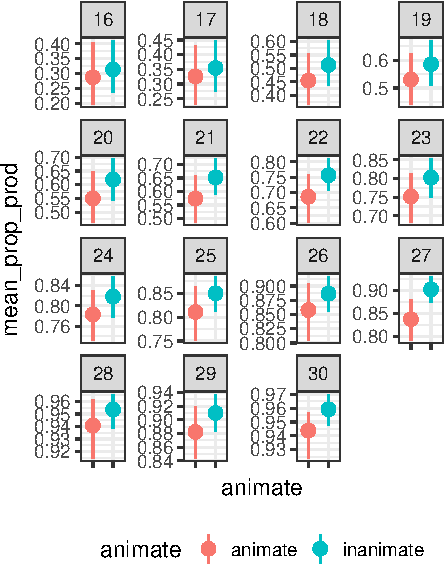
\includegraphics{figs/animacy_aoa-1} 
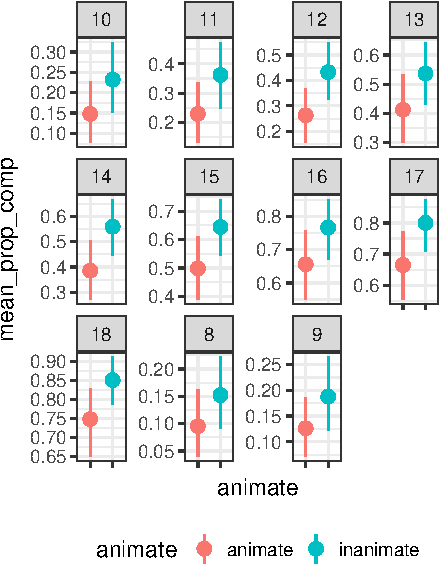
\includegraphics{figs/animacy_aoa-2} \end{CodeChunk}

\begin{CodeChunk}

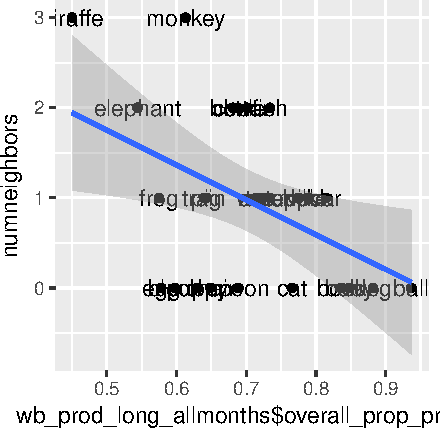
\includegraphics{figs/animacy_aoa_overall-1} 
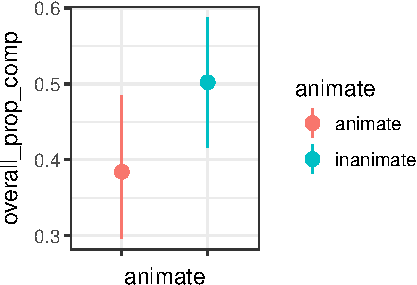
\includegraphics{figs/animacy_aoa_overall-2} 
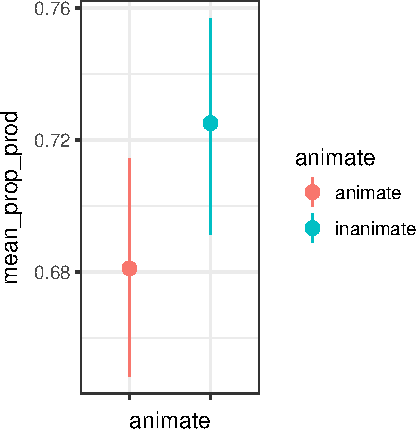
\includegraphics{figs/animacy_aoa_overall-3} 
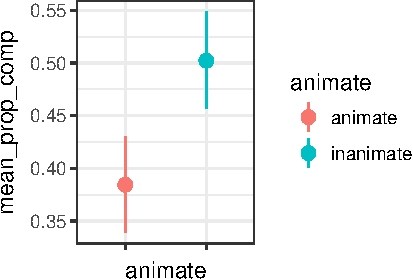
\includegraphics{figs/animacy_aoa_overall-4} \end{CodeChunk}

\section{Discussion}\label{discussion}

\section{Conclusion}\label{conclusion}

\section{Acknowledgements}\label{acknowledgements}

Place acknowledgments (including funding information) in a section at
the end of the paper.

(Gelman \& Markman, 1986, Tversky (1977), Kemp, Bernstein, \& Tenenbaum
(2005), Hahn, Chater, \& Richardson (2003), Pennington et al. (2014),
Szegedy et al. (2016), Firth (1957), Harris (1954), Russakovsky et al.
(2015))

\section{References}\label{references}

\setlength{\parindent}{-0.1in} \setlength{\leftskip}{0.125in} \noindent

\hypertarget{refs}{}
\hypertarget{ref-bergelson2016seedlings}{}
Bergelson, E. (2016a). Bergelson seedlings homebank corpus.
\url{http://doi.org/10.21415/T5PK6D}

\hypertarget{ref-bergelson2016seedlingsdatabrary}{}
Bergelson, E. (2016b). SEEDLingS corpus. Retrieved January 26, 2018,
from \url{https://nyu.databrary.org/volume/228}

\hypertarget{ref-firth1957synopsis}{}
Firth, J. R. (1957). A synopsis of linguistic theory, 1930-1955.
\emph{Studies in Linguistic Analysis}.

\hypertarget{ref-frank2017wordbank}{}
Frank, M. C., Braginsky, M., Yurovsky, D., \& Marchman, V. A. (2017).
Wordbank: An open repository for developmental vocabulary data.
\emph{Journal of Child Language}, \emph{44}(3), 677--694.

\hypertarget{ref-gelman1986categories}{}
Gelman, S. A., \& Markman, E. M. (1986). Categories and induction in
young children. \emph{Cognition}, \emph{23}(3), 183--209.

\hypertarget{ref-hahn2003similarity}{}
Hahn, U., Chater, N., \& Richardson, L. B. (2003). Similarity as
transformation. \emph{Cognition}, \emph{87}(1), 1--32.

\hypertarget{ref-harris1954distributional}{}
Harris, Z. S. (1954). Distributional structure. \emph{Word},
\emph{10}(2-3), 146--162.

\hypertarget{ref-kemp2005generative}{}
Kemp, C., Bernstein, A., \& Tenenbaum, J. B. (2005). A generative theory
of similarity. In \emph{Proceedings of the 27th annual conference of the
cognitive science society} (pp. 1132--1137).

\hypertarget{ref-pennington2014glove}{}
Pennington, J., Socher, R., \& Manning, C. (2014). Glove: Global vectors
for word representation. In \emph{Proceedings of the 2014 conference on
empirical methods in natural language processing (emnlp)} (pp.
1532--1543).

\hypertarget{ref-ILSVRC15}{}
Russakovsky, O., Deng, J., Su, H., Krause, J., Satheesh, S., Ma, S.,
\ldots{} Fei-Fei, L. (2015). ImageNet Large Scale Visual Recognition
Challenge. \emph{International Journal of Computer Vision (IJCV)},
\emph{115}(3), 211--252. \url{http://doi.org/10.1007/s11263-015-0816-y}

\hypertarget{ref-szegedy2016rethinking}{}
Szegedy, C., Vanhoucke, V., Ioffe, S., Shlens, J., \& Wojna, Z. (2016).
Rethinking the inception architecture for computer vision. In
\emph{Proceedings of the ieee conference on computer vision and pattern
recognition} (pp. 2818--2826).

\hypertarget{ref-tversky1977features}{}
Tversky, A. (1977). Features of similarity. \emph{Psychological Review},
\emph{84}(4), 327.

\end{document}
